\chapter[GLM]{Modelos Lineares Generalizados}

\begin{objetivos}
	Ao final desta unidade, o estudante deverá compreender os fundamentos dos Modelos Lineares Generalizados (GLM) aplicados à Modelagem de Distribuição de Espécies; ajustar modelos presença-background com família binomial; interpretar coeficientes, termos lineares e quadráticos; avaliar desempenho preditivo por AUC e TSS; gerar curvas de resposta parcial; projetar adequabilidade ambiental no espaço geográfico; e produzir mapas de adequabilidade atual para \textit{Dinizia excelsa} no bioma Amazônia.
\end{objetivos}

\section{Introdução}

Os Modelos Lineares Generalizados, conhecidos como GLM, representam uma das abordagens estatísticas mais clássicas e interpretáveis em Modelagem de Distribuição de Espécies. Em SDM, eles são frequentemente usados para relacionar registros de presença e ausência, ou presença e background, com variáveis ambientais preditoras \parencite{guisan2000,guisan2005predicting,guisan2017habitat}.

Em modelos presença-background, a resposta é binária: presença recebe valor 1 e background recebe valor 0. Embora pontos de background não sejam ausências verdadeiras, eles representam o conjunto de condições ambientais disponíveis dentro da área de calibração. Assim, o GLM estima a probabilidade relativa de ocorrência ou adequabilidade ambiental em função dos gradientes ambientais.

\begin{conceito}[title={\faBook\quad GLM em SDM}]
	Em SDM, um GLM binomial estima a relação entre a ocorrência da espécie e variáveis ambientais, usando uma função de ligação logit para transformar uma combinação linear de preditores em valores entre 0 e 1.
\end{conceito}

\section{Formulação matemática}

No caso binomial, seja \(Y_i\) uma variável resposta indicando presença ou background:

\[
Y_i =
\begin{cases}
	1, & \text{presença}\\
	0, & \text{background}
\end{cases}
\]

O GLM com ligação logit é definido por:

\begin{equationbox}
	\[
	\text{logit}(p_i)=
	\log\left(\frac{p_i}{1-p_i}\right)
	=
	\beta_0+\beta_1X_{1i}+\beta_2X_{2i}+...+\beta_kX_{ki}
	\]
	\[
	p_i=
	\frac{1}{1+\exp(-\eta_i)}
	\]
\end{equationbox}

em que \(p_i\) representa a adequabilidade estimada no pixel \(i\), \(X_k\) representa as variáveis ambientais e \(\beta_k\) representa os coeficientes estimados.

\begin{dica}[title={\faLightbulb\quad Termos quadráticos}]
	Em SDM, termos quadráticos são úteis porque permitem respostas unimodais, isto é, situações nas quais a espécie apresenta maior adequabilidade em valores intermediários de uma variável ambiental.
\end{dica}

\section{Preparação dos dados para GLM}

Nesta unidade, utilizamos a base presença-background construída na Unidade 5. As presenças correspondem aos registros finais de \textit{Dinizia excelsa}, enquanto os pontos de background foram amostrados dentro da área acessível \(M\). Essa base representa o conjunto de calibração dos modelos.

\rscriptfile{scripts/unidade06/01_estrutura_pastas.R}

\rscriptfile{scripts/unidade06/02_preparar_dados_glm.R}

\section{Ajuste do GLM}

O GLM é ajustado com família binomial e ligação logit. Para aumentar a flexibilidade ecológica, o modelo inclui termos lineares e quadráticos das variáveis selecionadas. Antes do ajuste, as variáveis ambientais são padronizadas para média zero e desvio-padrão um, reduzindo problemas numéricos e facilitando a comparação entre coeficientes.

\rscriptfile{scripts/unidade06/03_ajustar_glm_dinizia.R}

\begin{figure}[H]
	\centering
	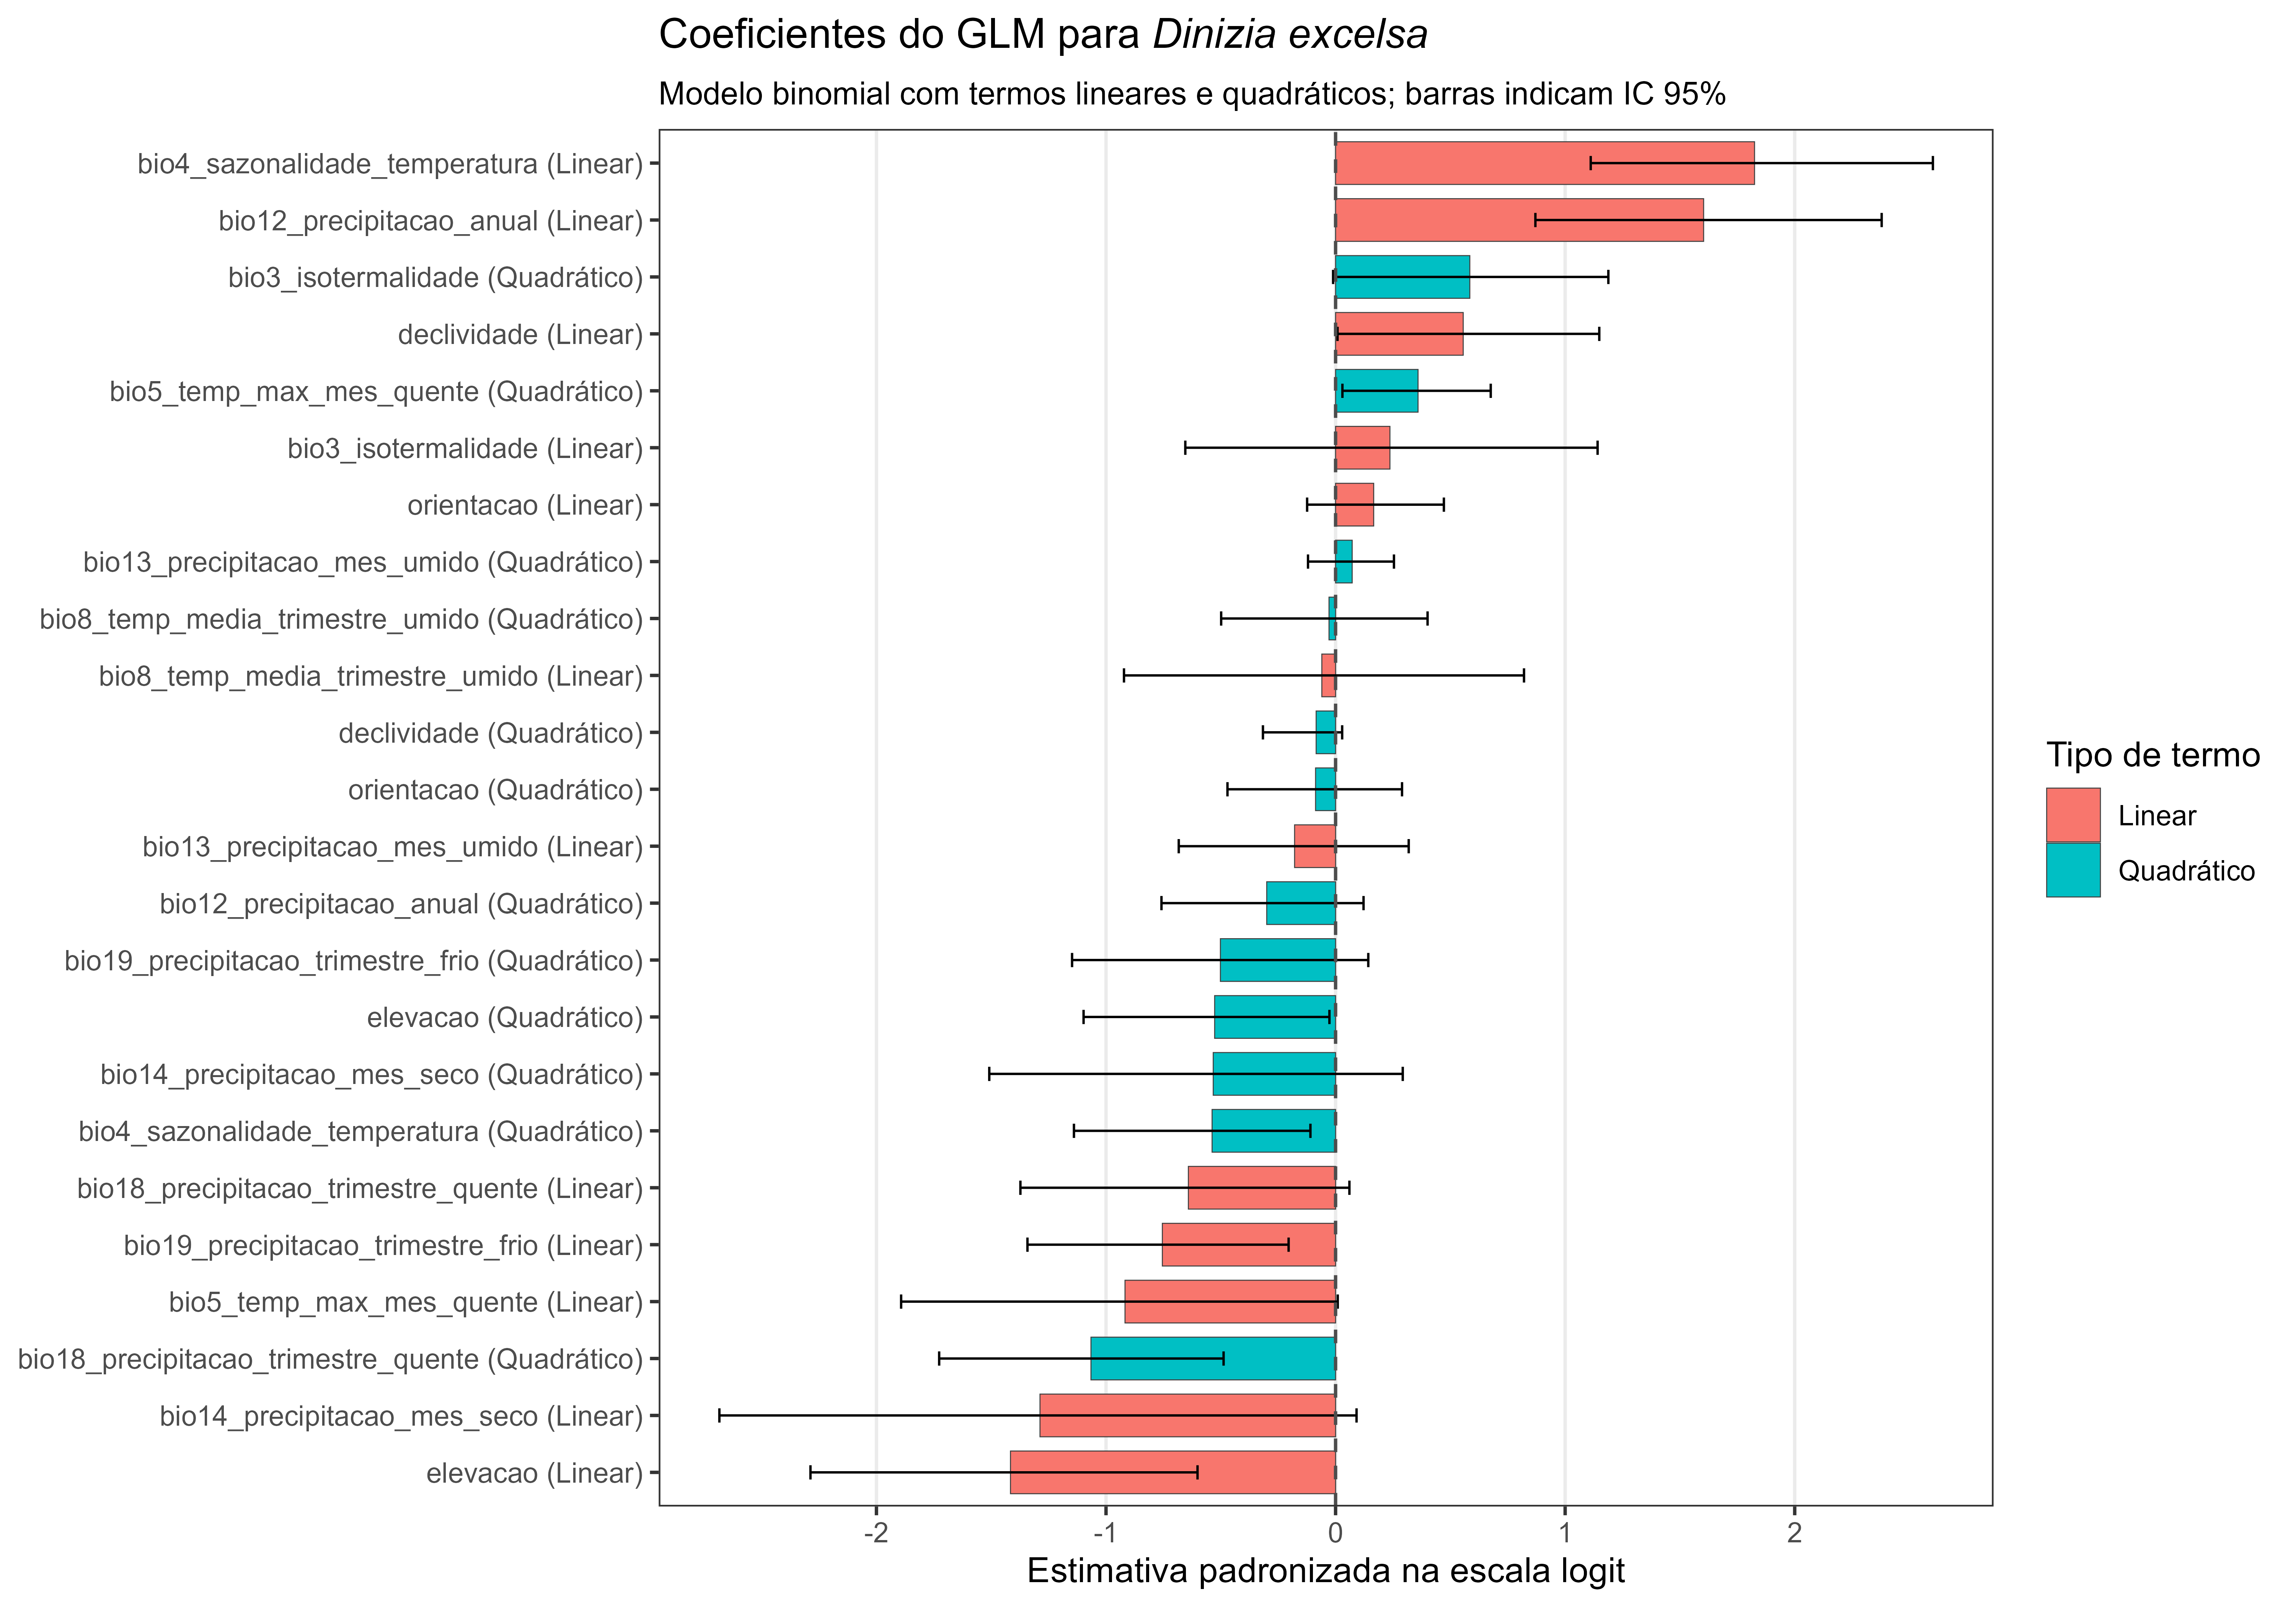
\includegraphics[width=0.88\textwidth]{figuras/unidade06/unidade06_coeficientes_glm.png}
	\caption{Coeficientes estimados pelo GLM para \textit{Dinizia excelsa}. Valores positivos indicam associação positiva com a adequabilidade relativa; valores negativos indicam associação negativa, considerando as demais variáveis do modelo.}
	\label{fig:unidade06_coeficientes_glm}
\end{figure}

\section{Avaliação do modelo}

A avaliação do GLM é feita usando AUC, TSS, sensibilidade, especificidade e matriz de confusão. AUC resume a capacidade de discriminação do modelo ao longo de diferentes limiares; TSS combina sensibilidade e especificidade em um único índice. Como trabalhamos com presença-background, essas métricas devem ser interpretadas como indicadores comparativos, não como validação absoluta da distribuição real da espécie.

\rscriptfile{scripts/unidade06/04_avaliar_glm_dinizia.R}

\begin{figure}[H]
	\centering
	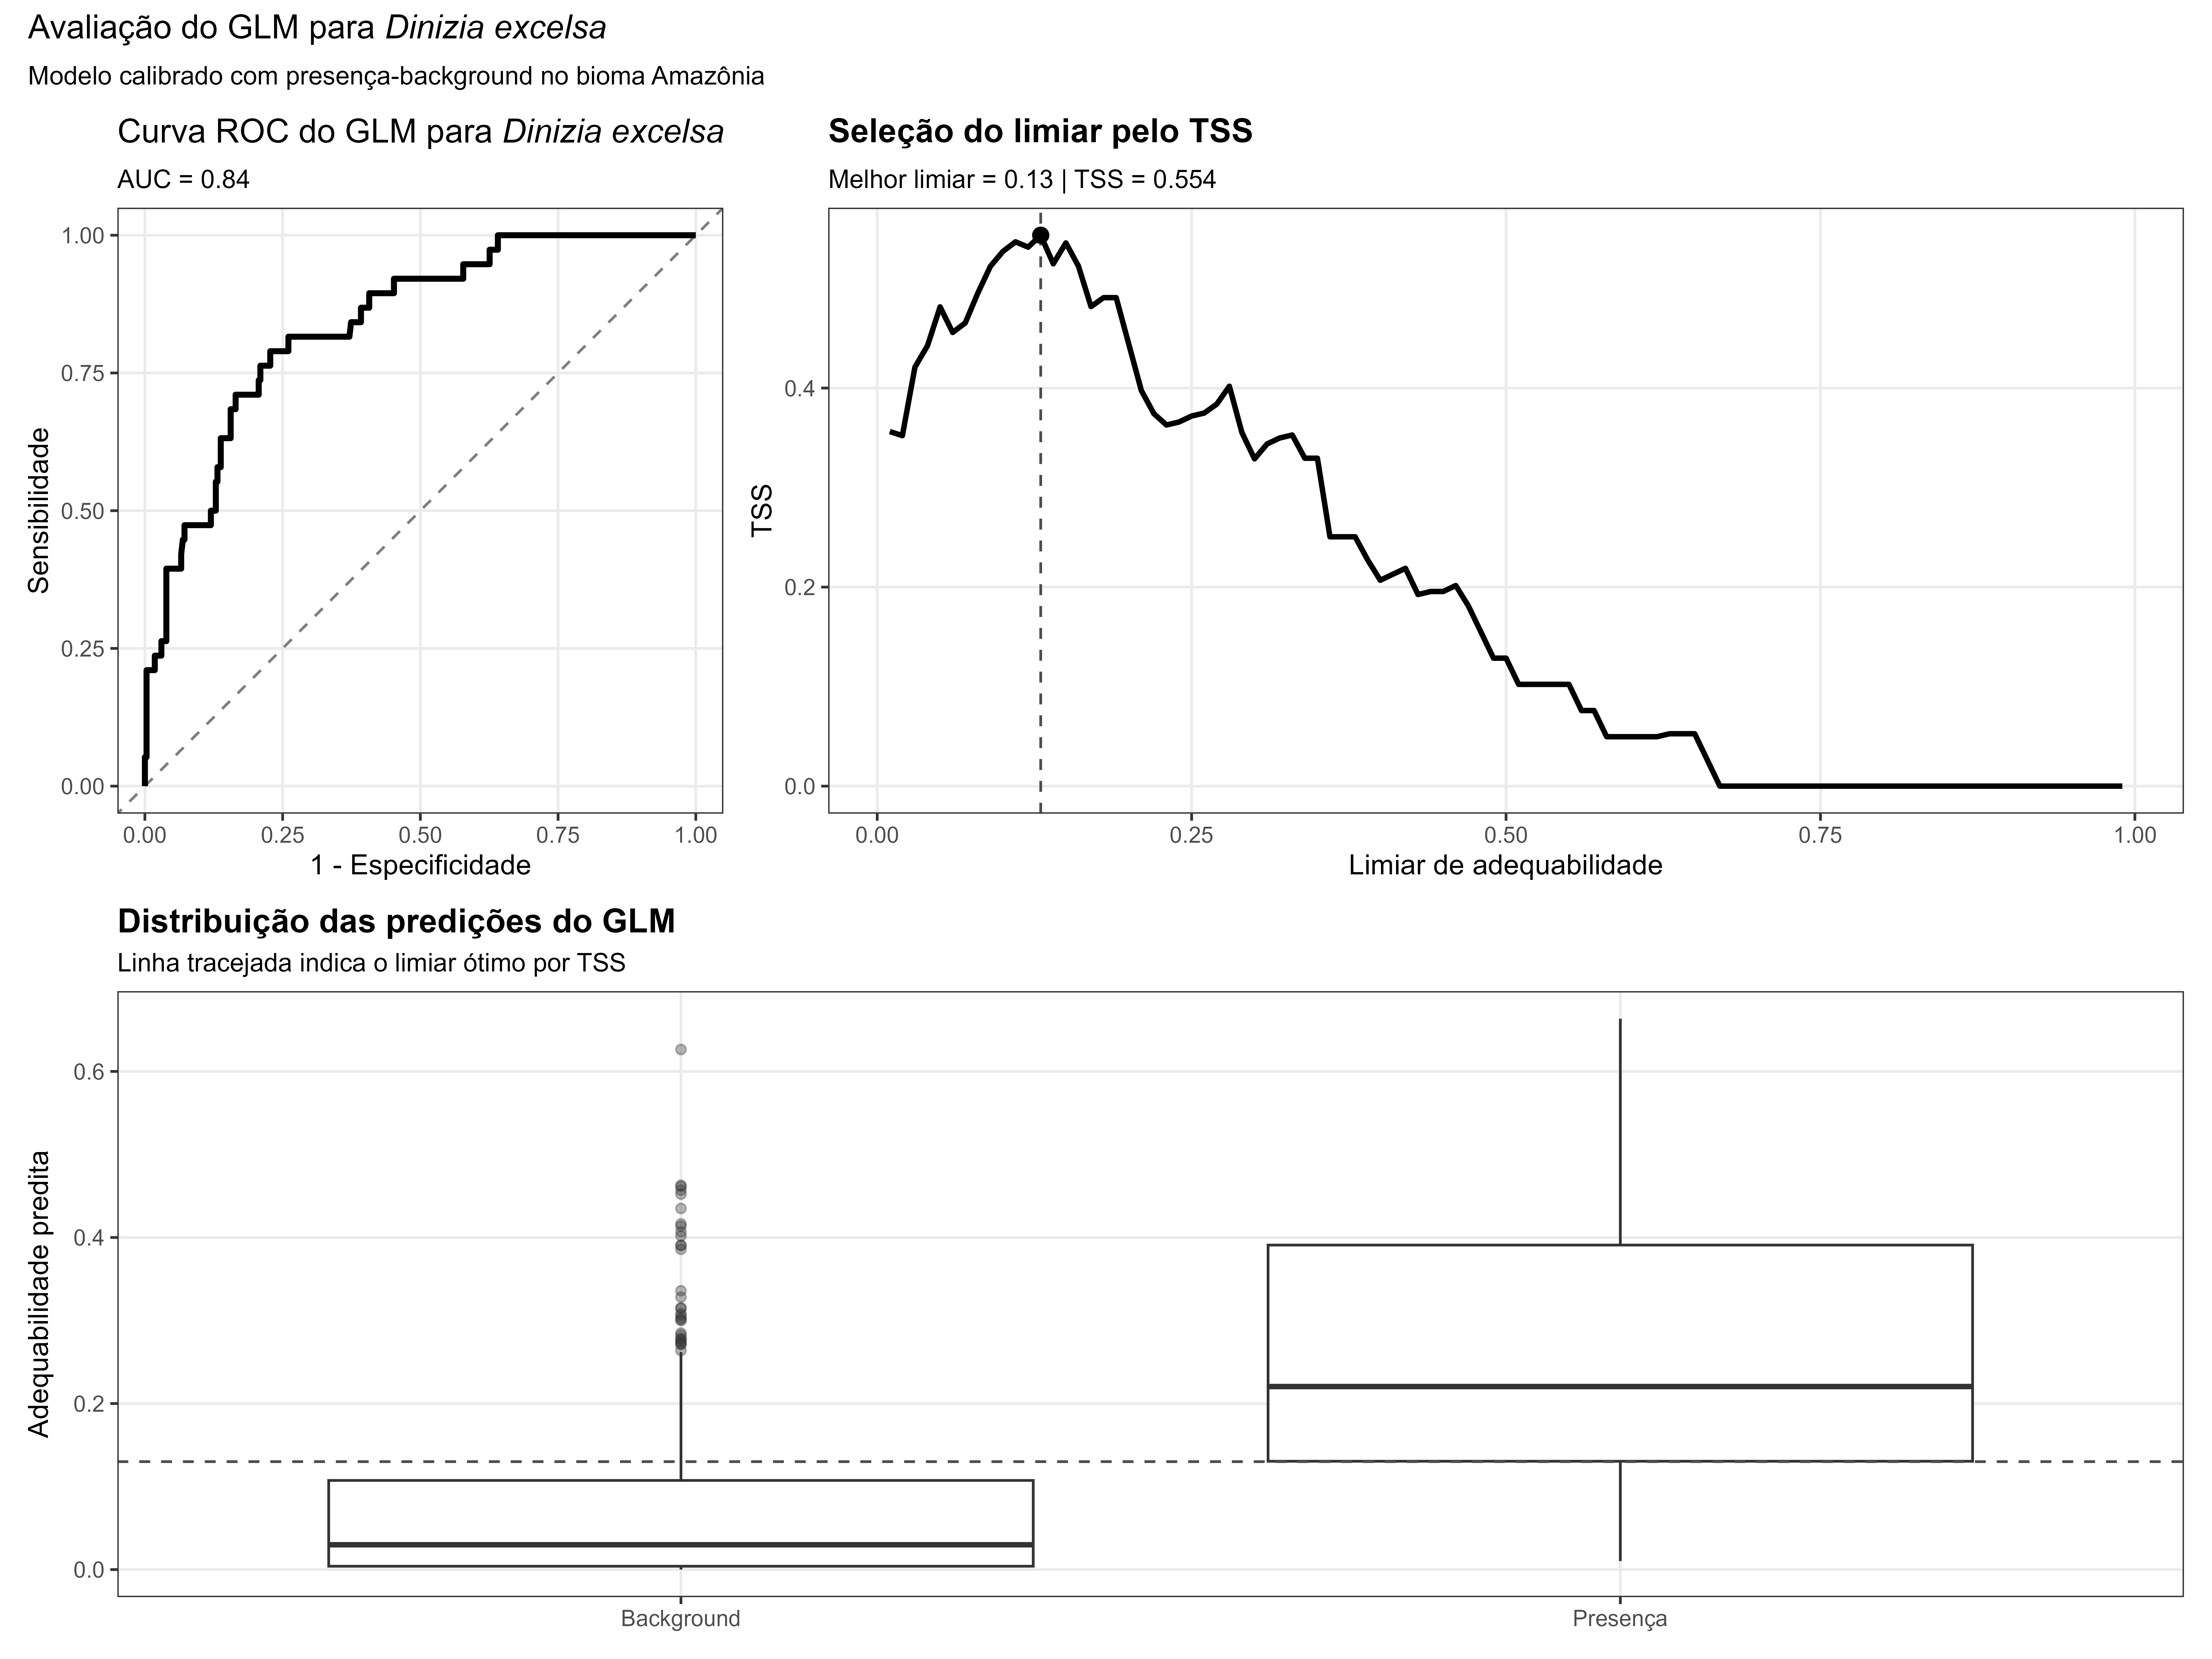
\includegraphics[width=0.82\textwidth]{figuras/unidade06/unidade06_avaliacao_glm_patchwork.png}
	\caption{Curva ROC do GLM ajustado para \textit{Dinizia excelsa}.}
	\label{fig:unidade06_roc_glm}
\end{figure}

\section{Curvas de resposta parcial}

As curvas de resposta parcial mostram como a adequabilidade estimada varia ao longo de cada variável ambiental, mantendo as demais constantes. Elas são essenciais para interpretar ecologicamente o comportamento do modelo.

\rscriptfile{scripts/unidade06/06_curvas_resposta_glm.R}

\begin{figure}[H]
	\centering
	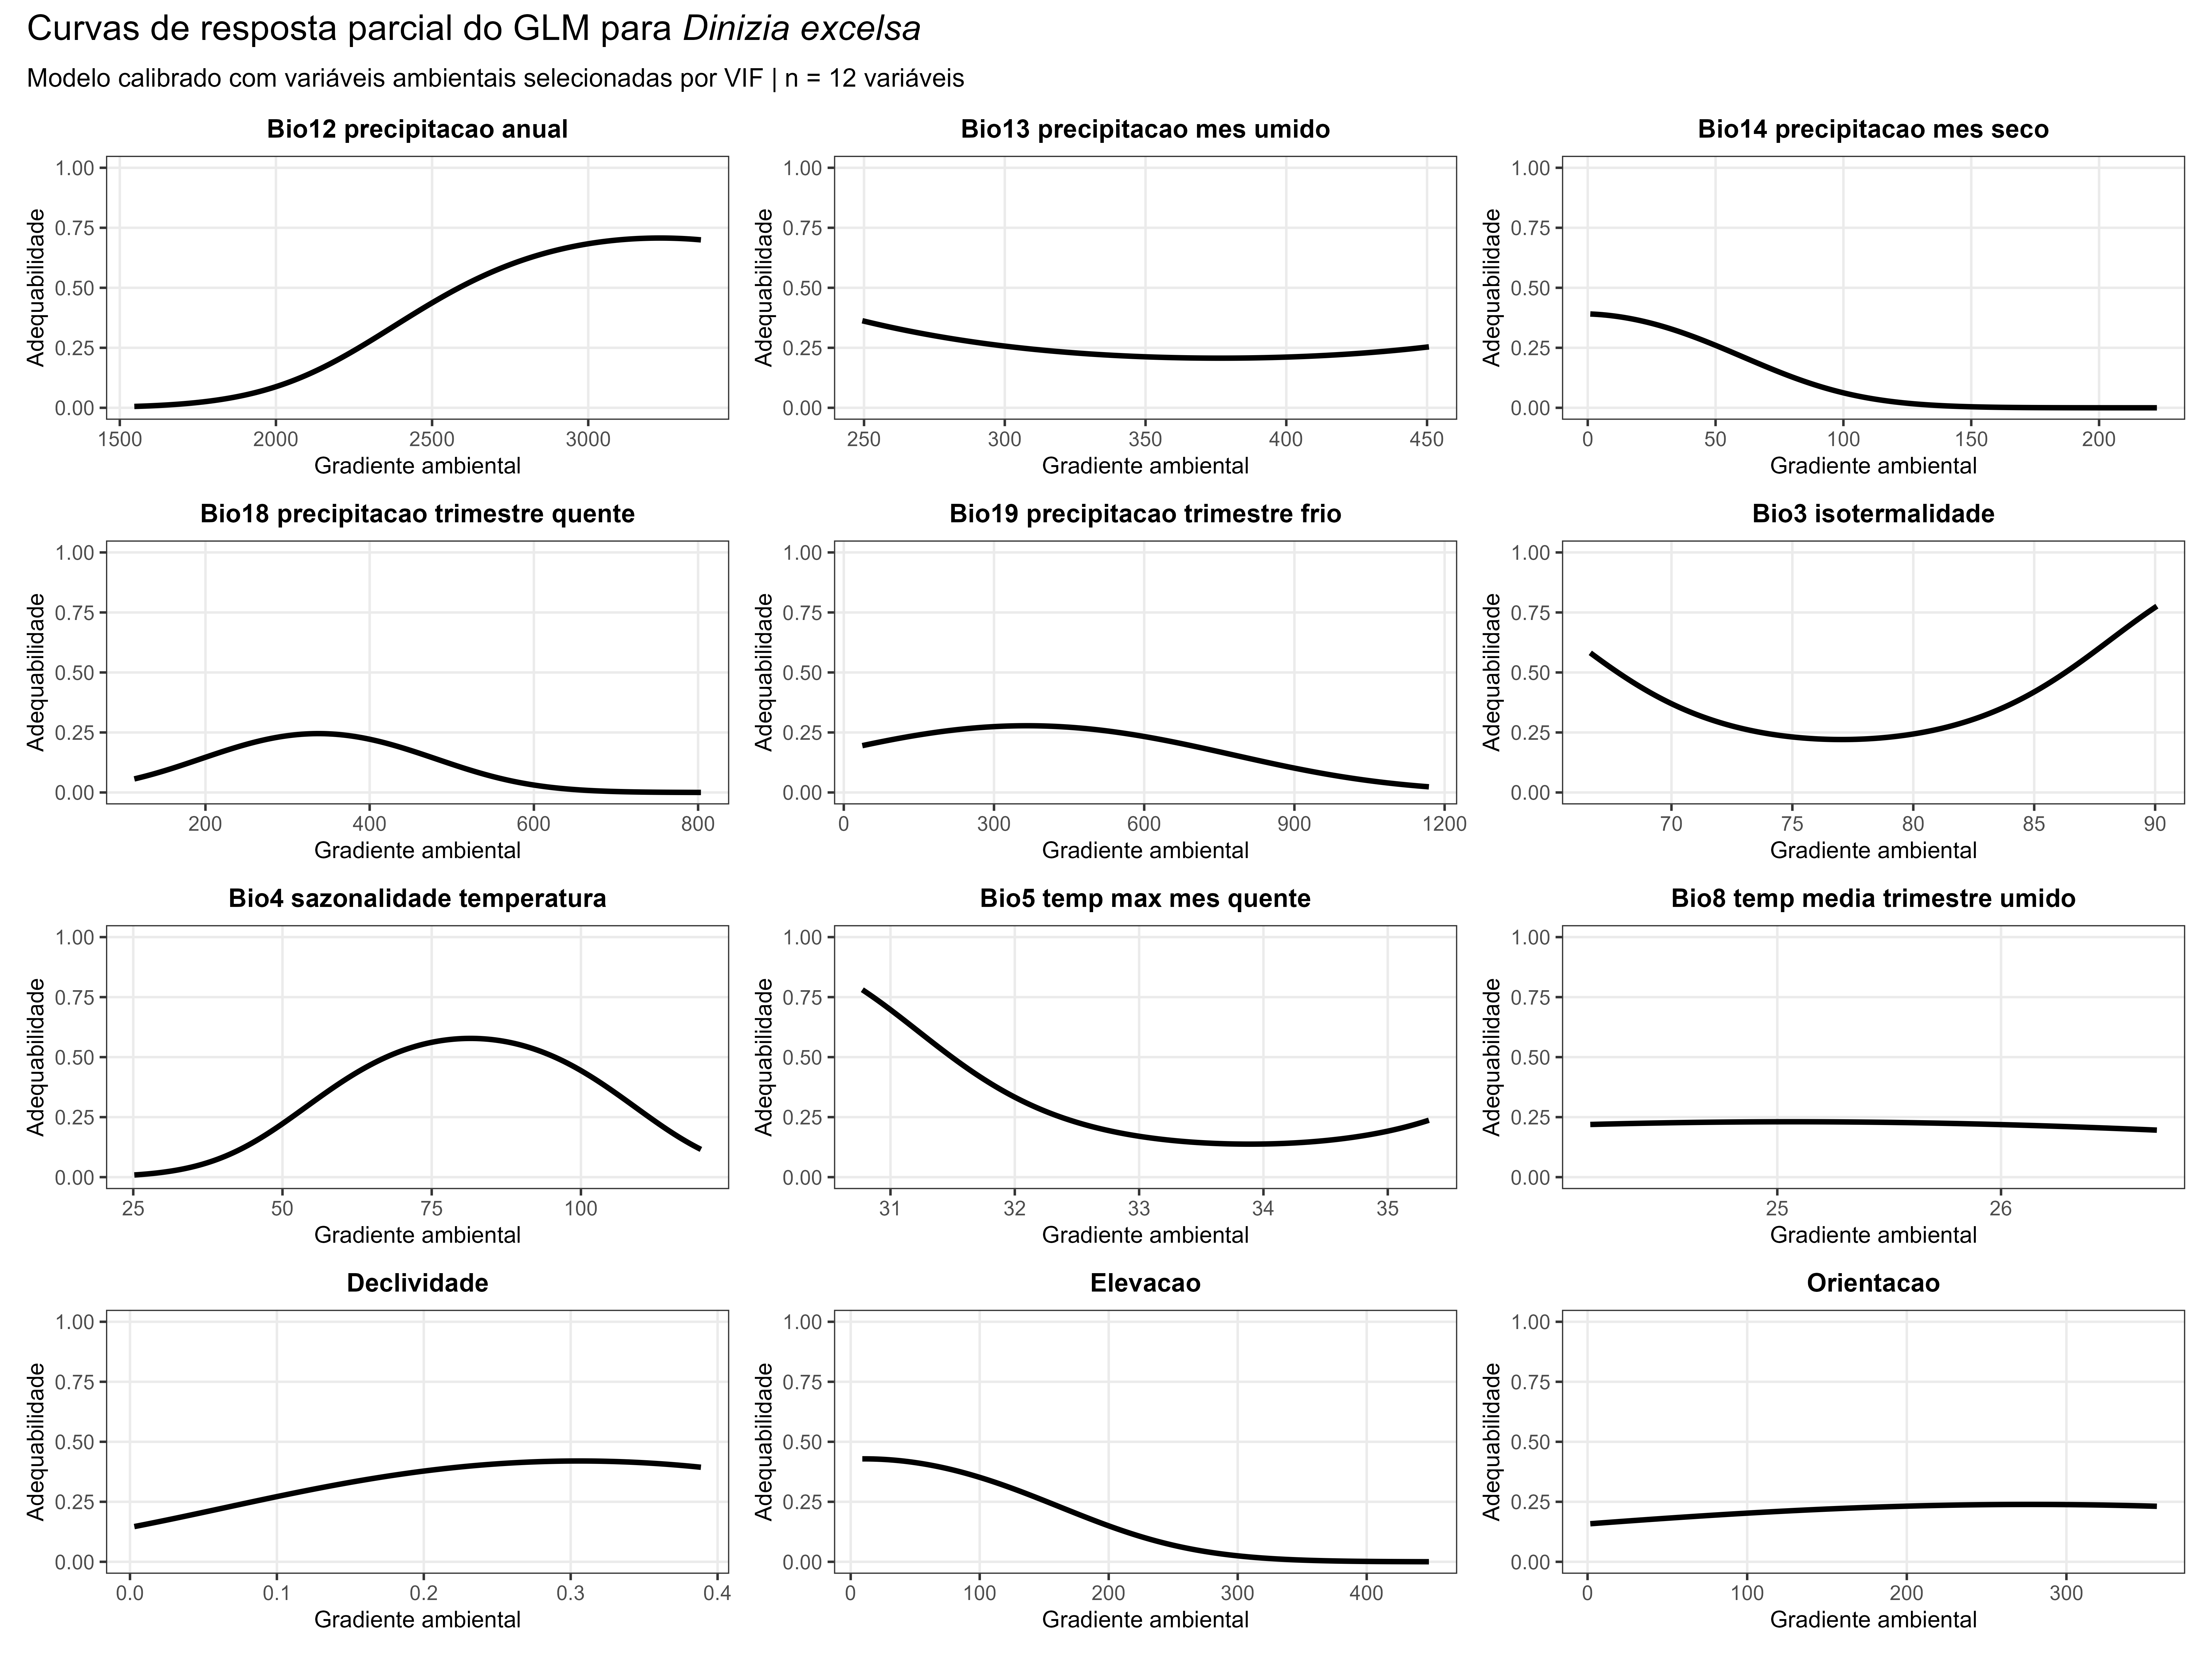
\includegraphics[width=0.96\textwidth]{figuras/unidade06/unidade06_curvas_resposta_glm.png}
	\caption{Curvas de resposta parcial do GLM para as variáveis ambientais selecionadas.}
	\label{fig:unidade06_curvas_resposta}
\end{figure}

\section{Projeção espacial da adequabilidade atual}

Após o ajuste e avaliação, o GLM é projetado para a pilha ambiental da área de estudo. O resultado é um mapa contínuo de adequabilidade ambiental atual para \textit{Dinizia excelsa}.

\rscriptfile{scripts/unidade06/05_predicao_espacial_glm.R}

\begin{figure}[H]
	\centering
	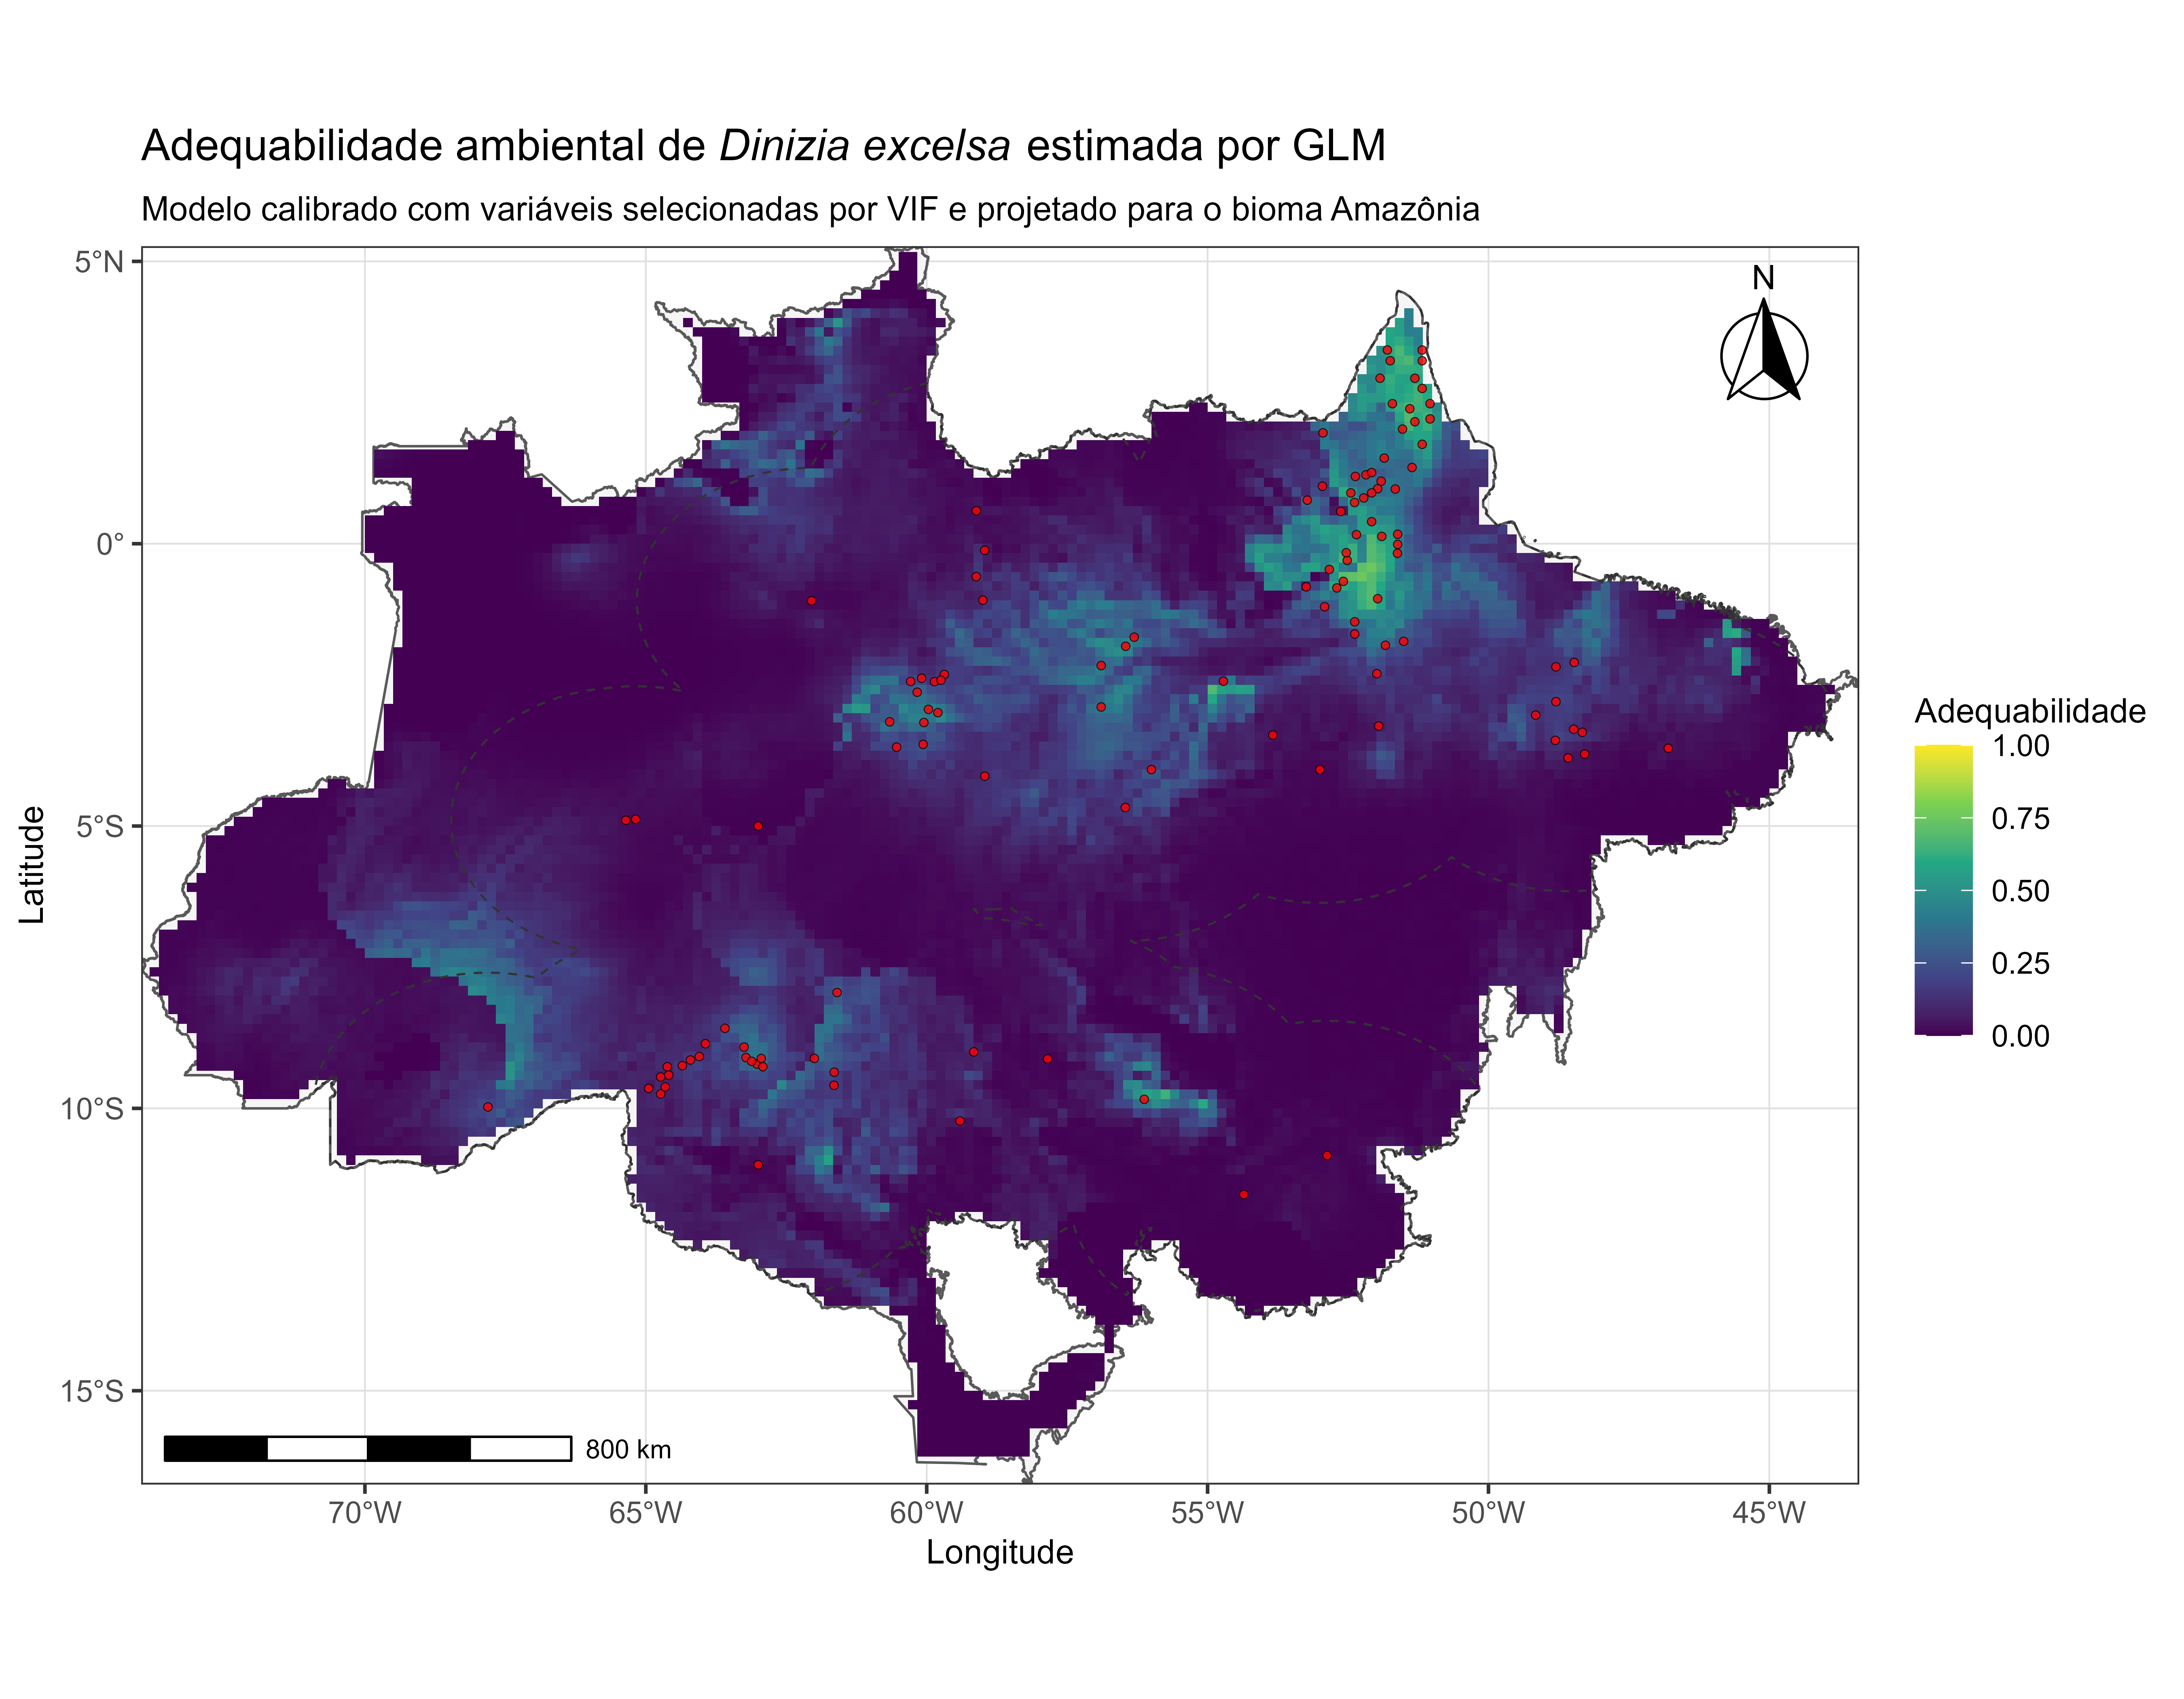
\includegraphics[width=0.90\textwidth]{figuras/unidade06/unidade06_adequabilidade_glm.png}
	\caption{Mapa de adequabilidade ambiental atual de \textit{Dinizia excelsa} estimado por GLM.}
	\label{fig:unidade06_adequabilidade_glm}
\end{figure}

\section{Pipeline completo}

\rscriptfile{scripts/unidade06/07_pipeline_glm.R}

\section{Síntese da unidade}

O GLM é um modelo simples, interpretável e robusto para iniciar análises de SDM. Embora menos flexível que GAM, Random Forest, BRT ou Maxent, ele permite compreender explicitamente a relação entre ocorrência e gradientes ambientais. Por isso, é uma ferramenta fundamental em materiais didáticos, análises exploratórias e estudos que priorizam transparência e interpretação ecológica.

\begin{conceito}[title={\faBook\quad Mensagem central}]
	O GLM é uma ponte entre estatística clássica e SDM moderna: simples o suficiente para interpretação ecológica, mas poderoso o suficiente para produzir mapas de adequabilidade ambiental quando bem calibrado.
\end{conceito}

\section{Exercícios de fixação}

\begin{enumerate}
	\item Explique por que a família binomial é apropriada para modelos presença-background.
	\item O que representa a função logit em um GLM?
	\item Por que termos quadráticos são úteis em SDM?
	\item Diferencie coeficiente positivo e coeficiente negativo em um GLM.
	\item Explique a diferença entre AUC e TSS.
	\item Por que curvas de resposta parcial são importantes para interpretação ecológica?
	\item Quais limitações devem ser consideradas ao usar GLM em projeções espaciais?
\end{enumerate}

% ============================================================
% UNIDADE 7
% ============================================================

